\begin{quote}
\textbf{Alvin Toffler}: If overstimulation at the sensory level
increases the distortion with which we perceive reality, cognitive
overstimulation interferes with our ability to `think.'
\end{quote}

%% \begin{center}
%% 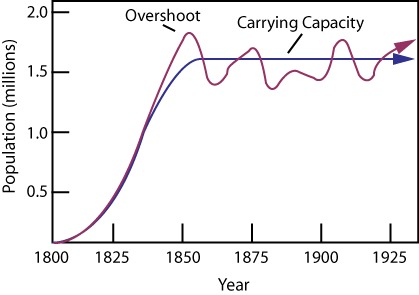
\includegraphics[width=.65\textwidth]{../pictures/carrying_capacity.jpg} \\
%% Image from
%% \href{http://missbakersbiologyclasswiki.wikispaces.com/Ecology+Study+Guide}{Miss
%% Baker's Biology Class Wiki} (CC-By-NC-SA).
%% \end{center}

At times, a facilitator or participant in the peer-learning enterprise
may feel he or she is over-contributing -- or, perhaps more likely, that
others are under-contributing -- or that someone else is railroading an
idea or dominating the discussion. If this happens, take a step back and
observe the dynamics of involvement. Ask questions and let others
answer. Especially if you start to feel the symptoms of burnout, it's
important that you find the level of engagement that allows you to
participate at a level that is feasible for maintaining progress toward
the project's goal. Lead by example -- but make sure it's someplace you,
and others, actually want to go! This could be a good time to revisit
the group's roadmap and see if you can figure out and clarify to others
what concrete goal you're working towards. Remember that you can also
change the ``landscape'' by making it easier for other people to get
involved -- for example, by explaining what you're trying to do in a
clear manner. Watch for opportunities to step back, watch, listen. Try
to be mindful of phases when active or quiet involvement would be more
helpful to the individual and the group. It's also helpful to let anyone
who has taken on a facilitation role know if you're stepping back
temporarily. Then, when the time is right, step back in and get to work!
